\documentclass[bwprint]{gmcmthesis}
\usepackage{amsmath}
\numberwithin{figure}{section}
\renewcommand{\thefigure}{\arabic{section}-\arabic{figure}} 
% \documentclass[withoutpreface,bwprint]{cumcmthesis}
% 去掉封面与编号页

\title{中国研究生数学建模竞赛论文标题}
\baominghao{No.00000001} %参赛队号
\schoolname{XX大学/学院}%学校名称
\membera{队员A} %队员A
\memberb{队员B} %队员B
\memberc{队员C} %队员C
\begin{document}
 \maketitle
 \begin{abstract}
第一段:针对自己选择的题目,说明自己用了什么方法来解决的(这类题属于哪种典型的问题),其中利用了哪些关键的算法,再说出自己的所建模型的创新点。没有创新点,也可以说自己所建的模型相比较于其它的是一个很好的方案。

第二段:问题一中,针对具体问题,进行分析和求解,几句话介绍自己是怎么解决的,有数字结果的也可以直接贴结果。

第三段:问题二中,类比于第二段。

第四段:问题三中,类比于第三段。

第五段:问题四中,类比于第四段。

第六段:如果有问题五,类比于第五段,没有就结束,也可以写一下团队的想法。






\keywords{针对具体的问题列一到两个关键字\quad  建模算法列出\quad }
\end{abstract}

%\pagestyle{plain}

%目录
\tableofcontents

\section{问题重述}
问题重述问题重述问题重述问题重述问题重述问题重述问题重述问题重述问题重述问题重述问题重述问题重述问题重述问题重述问题重述问题重述问题重述。


\begin{figure}[!h]
\centering
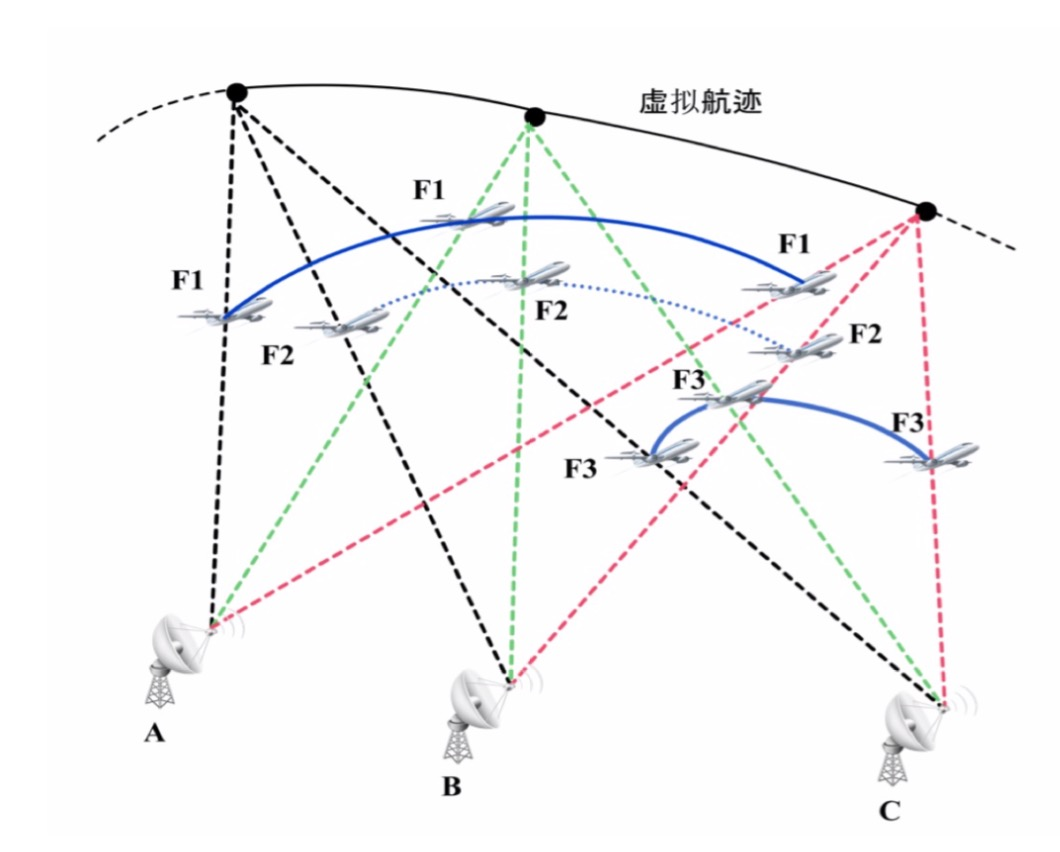
\includegraphics[width=.7\textwidth]{test.jpg}
\caption{对雷达实施距离多假目标欺骗干扰示意图}
\label{fig1}
\end{figure}
\begin{figure}[!h]
\centering
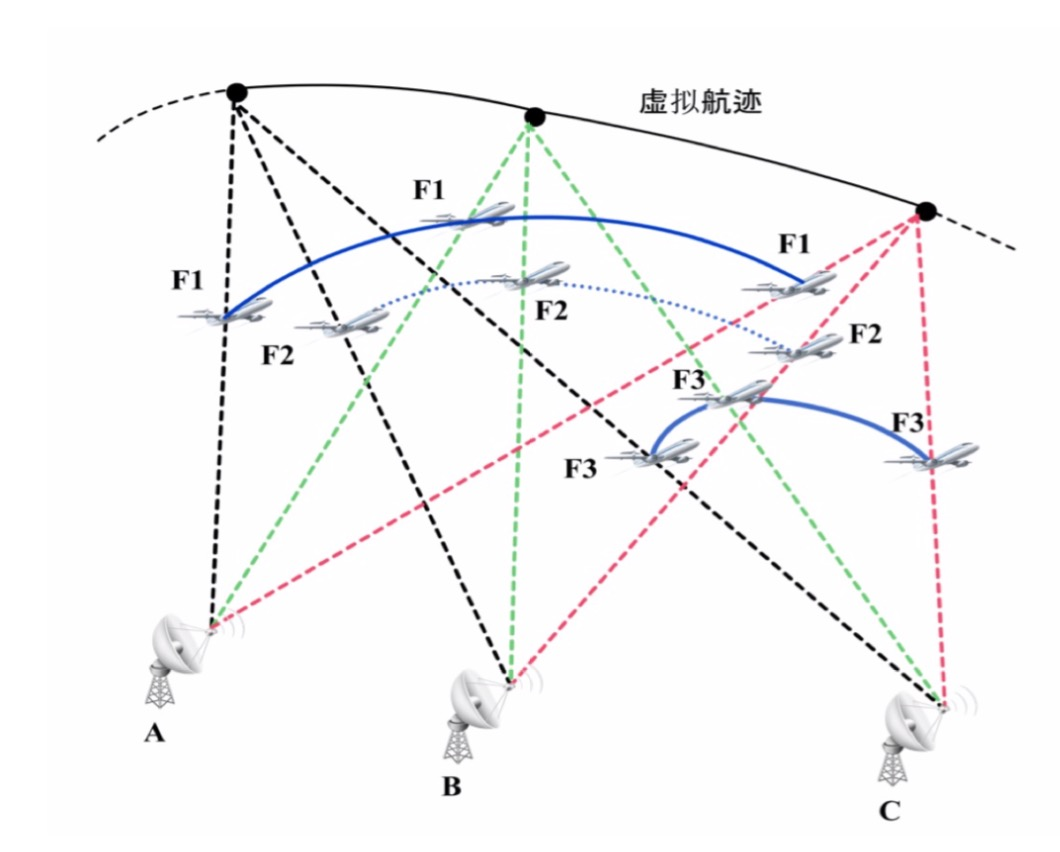
\includegraphics[width=.7\textwidth]{test.jpg}
\caption{对雷达实施距离多假目标欺骗干扰示意图}
\label{fig1}
\end{figure}

\section{模型假设}
模型假设模型假设模型假设模型假设模型假设模型假设模型假设模型假设模型假设模型假设模型假设模型假设模型假设模型假设模型假设模型假设模型假设模型假设。
\begin{figure}[!h]
\centering
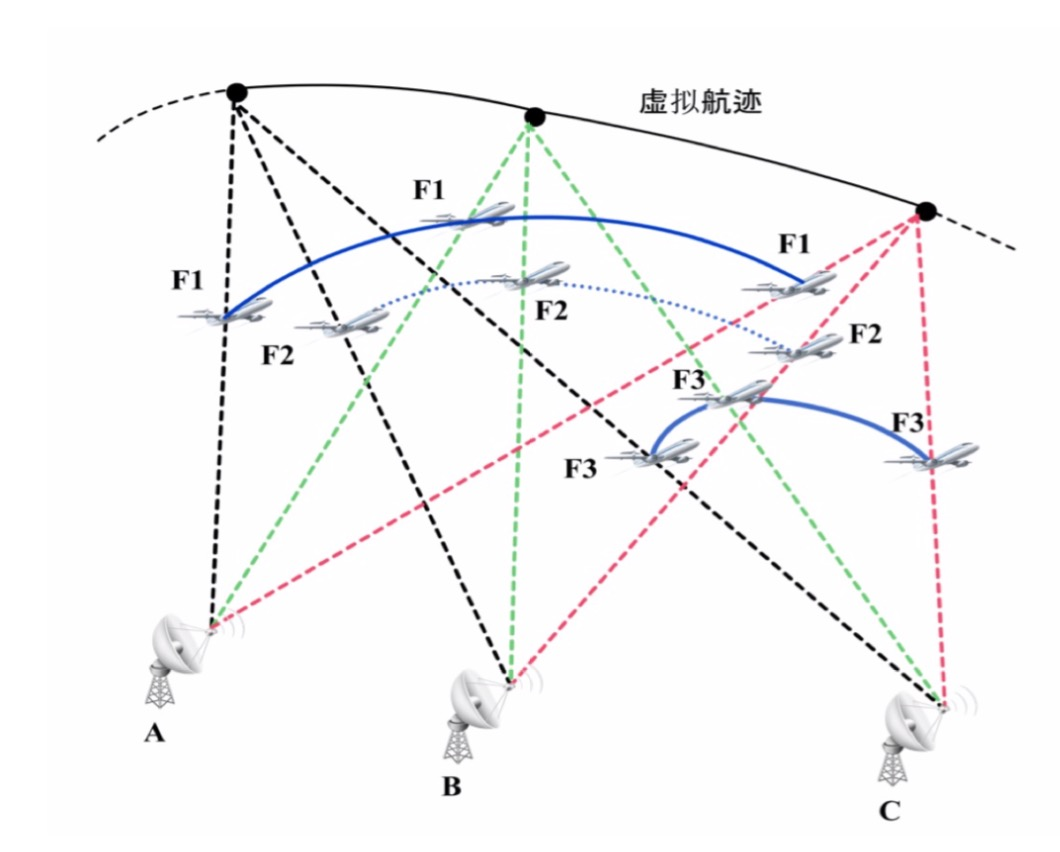
\includegraphics[width=.7\textwidth]{test.jpg}
\caption{对雷达实施距离多假目标欺骗干扰示意图}
\label{fig1}
\end{figure}

\begin{figure}[!h]
\centering
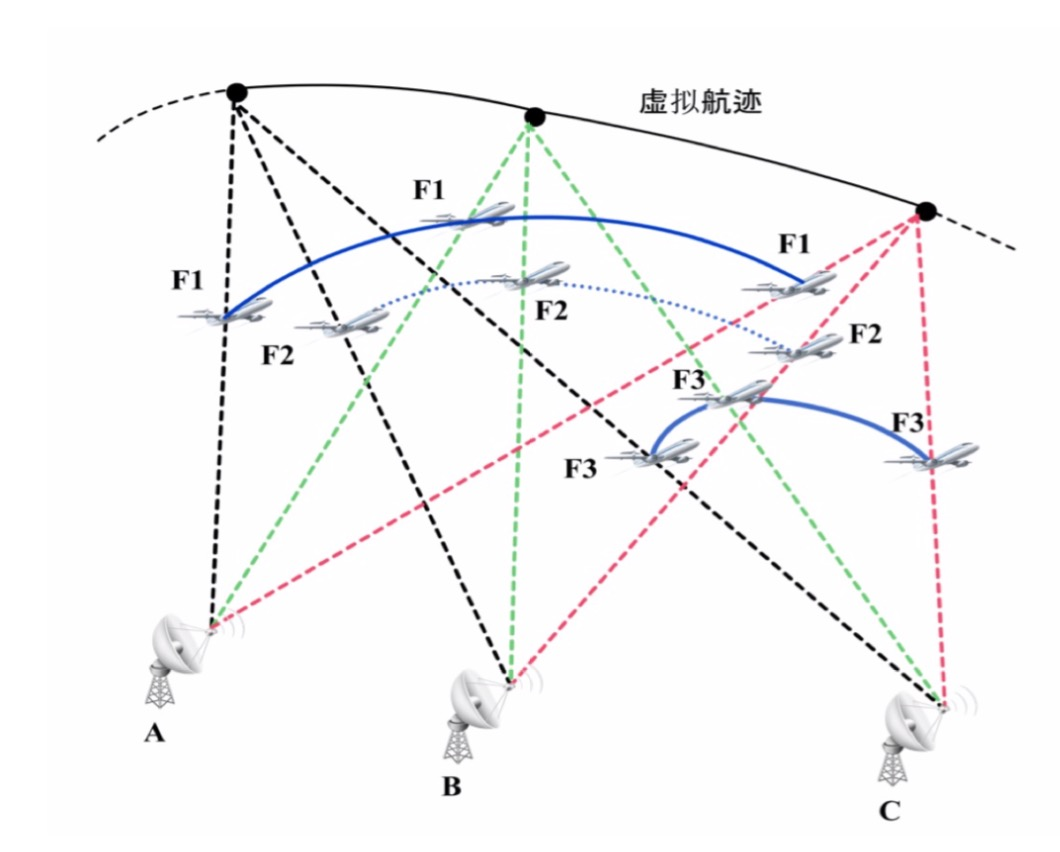
\includegraphics[width=.7\textwidth]{test.jpg}
\caption{对雷达实施距离多假目标欺骗干扰示意图}
\label{fig1}
\end{figure}

\begin{figure}[!h]
\centering
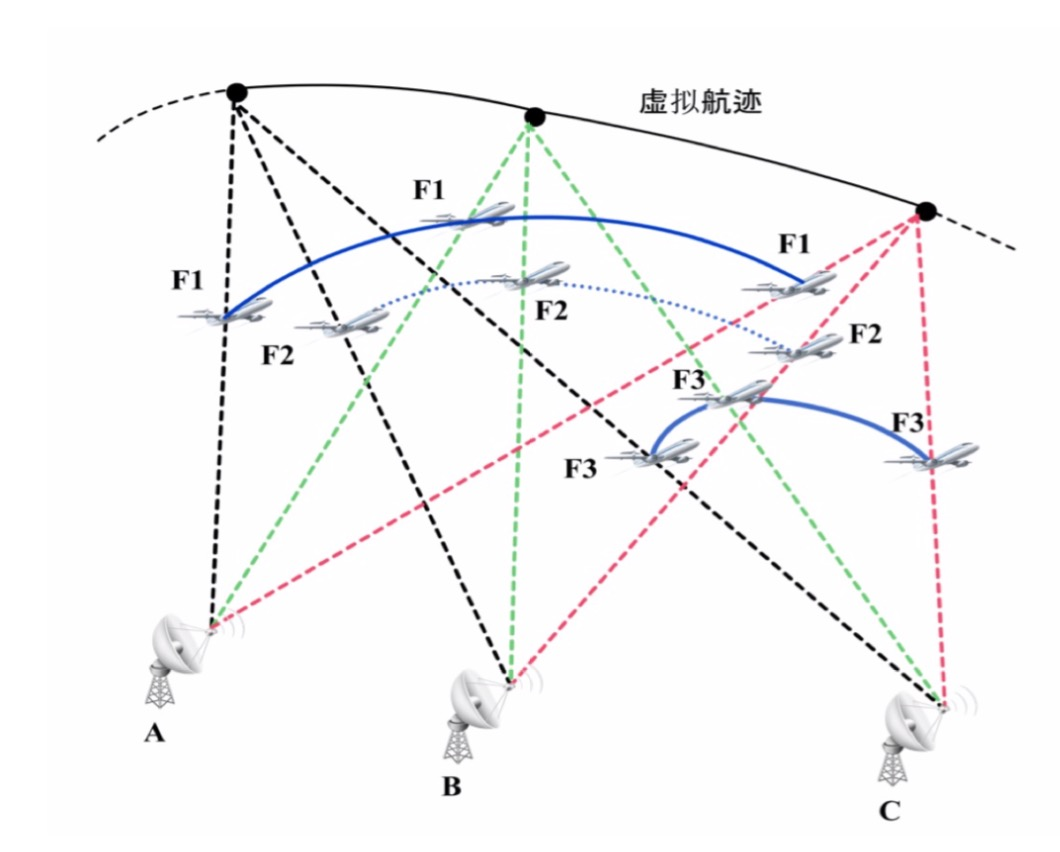
\includegraphics[width=.7\textwidth]{test.jpg}
\caption{对雷达实施距离多假目标欺骗干扰示意图}
\label{fig1}
\end{figure}
\section{符号说明}
符号说明符号说明符号说明符号说明符号说明符号说明符号说明符号说明符号说明符号说明符号说明符号说明符号说明符号说明符号说明符号说明符号说明。
\section{问题的分析}
\subsection{问题一 xxx}
\subsubsection{问题描述和分析}
问题的分析问题的分析问题的分析问题的分析问题的分析问题的分析问题的分析问题的分析问题的分析问题的分析问题的分析问题的分析问题的分析问题的分析。
\subsubsection{模型建立与求解}
模型建立与求解模型建立与求解模型建立与求解模型建立与求解模型建立与求解模型建立与求解模型建立与求解模型建立与求解模型建立与求解模型建立与求解模型建立与求解。


\subsection{问题二 xxx}
\subsubsection{问题描述和分析}
问题的分析问题的分析问题的分析问题的分析问题的分析问题的分析问题的分析问题的分析问题的分析问题的分析问题的分析问题的分析问题的分析问题的分析。
\subsubsection{模型建立与求解}
模型建立与求解模型建立与求解模型建立与求解模型建立与求解模型建立与求解模型建立与求解模型建立与求解模型建立与求解模型建立与求解模型建立与求解模型建立与求解。

\subsection{问题三 xxx}
\subsubsection{问题描述和分析}
问题的分析问题的分析问题的分析问题的分析问题的分析问题的分析问题的分析问题的分析问题的分析问题的分析问题的分析问题的分析问题的分析问题的分析。
\subsubsection{模型建立与求解}
模型建立与求解模型建立与求解模型建立与求解模型建立与求解模型建立与求解模型建立与求解模型建立与求解模型建立与求解模型建立与求解模型建立与求解模型建立与求解。

\subsection{问题四 xxx}
\subsubsection{问题描述和分析}
问题的分析问题的分析问题的分析问题的分析问题的分析问题的分析问题的分析问题的分析问题的分析问题的分析问题的分析问题的分析问题的分析问题的分析。
\subsubsection{模型建立与求解}
模型建立与求解模型建立与求解模型建立与求解模型建立与求解模型建立与求解模型建立与求解模型建立与求解模型建立与求解模型建立与求解模型建立与求解模型建立与求解。

\section{模型的评价}
\subsection{模型的优点}
模型的优点模型的优点模型的优点模型的优点模型的优点模型的优点模型的优点模型的优点模型的优点模型的优点模型的优点模型的优点模型的优点模型的优点。
\subsection{模型的缺点}
模型的缺点模型的缺点模型的缺点模型的缺点模型的缺点模型的缺点模型的缺点模型的缺点模型的缺点模型的缺点模型的缺点模型的缺点模型的缺点模型的缺点。



\section{写作参考格式}
写作过程中可能要用到一些格式参考,正式写作的时候,可以直接将这一章删掉即可。

\textbf{无序列表格式}
\begin{itemize}
\item 无序列表1
\item 无序列表2
\item 无序列表3
\item 无序列表4
\end{itemize}


\textbf{表格格式}

\begin{tabular}{cc}
 \hline
 \makebox[0.4\textwidth][c]{符号}	&  \makebox[0.5\textwidth][c]{意义} \\ \hline
 D	    & 宽度(cm) \\ \hline
 L	    & 长度(cm)  \\ \hline
\end{tabular}


%
%\textbf{图片格式}
%\begin{figure}[h]
%\centering
%\includegraphics[width=5cm]{xxx.jpg}
%\caption{图片标题}
%\end{figure}

\section{参考文献}
%参考文献
\begin{thebibliography}{1.2}%宽度9
\setlength{\itemsep}{-2mm}
 \bibitem{bib:one} 
 韩中庚. 数学建模方法及其应用[M]. 高等教育出版社, 2005.
 \bibitem{bib:two}
 韩中庚. 数学建模方法及其应用[M]. 高等教育出版社, 2005.
  \bibitem{bib:two}
 韩中庚. 数学建模方法及其应用[M]. 高等教育出版社, 2005.
\end{thebibliography}

\newpage
%附录
\appendix
\section{程序代码}
%设置不同语言即可。
\begin{lstlisting}[language=Matlab] 
kk=2;[mdd,ndd]=size(dd);
while ~isempty(V)
[tmpd,j]=min(W(i,V));tmpj=V(j);
for k=2:ndd
[tmp1,jj]=min(dd(1,k)+W(dd(2,k),V));
tmp2=V(jj);tt(k-1,:)=[tmp1,tmp2,jj];
end
tmp=[tmpd,tmpj,j;tt];[tmp3,tmp4]=min(tmp(:,1));
if tmp3==tmpd, ss(1:2,kk)=[i;tmp(tmp4,2)];
else,tmp5=find(ss(:,tmp4)~=0);tmp6=length(tmp5);
if dd(2,tmp4)==ss(tmp6,tmp4)
ss(1:tmp6+1,kk)=[ss(tmp5,tmp4);tmp(tmp4,2)];
else, ss(1:3,kk)=[i;dd(2,tmp4);tmp(tmp4,2)];
end;end
dd=[dd,[tmp3;tmp(tmp4,2)]];V(tmp(tmp4,3))=[];
[mdd,ndd]=size(dd);kk=kk+1;
end; S=ss; D=dd(1,:);
 \end{lstlisting}


\end{document} 